\documentclass[10pt]{beamer}

% THEME
\usetheme{CambridgeUS}
\usecolortheme{spruce}
\usefonttheme{professionalfonts}

% PACKAGES
\usepackage{graphicx}
\usepackage{booktabs}
\usepackage{amsmath}
\usepackage{array}
\usepackage{tikz}
\usetikzlibrary{arrows.meta,positioning}
\usepackage{hyperref}

\graphicspath{{figures/}}

\title{Reproduction of CDNMF:\\Contrastive Deep NMF for Community Detection}
\subtitle{Lab 1 --- Paper Reproduction}
\author{Group 4}
\date{}

\begin{document}

% TITLE SLIDE
\begin{frame}
\titlepage
\vspace{-0.5cm}
\centering
\textbf{Indian Institute of Information Technology, Vadodara} \\[0.15cm]
\textbf{International Campus Diu (IIITV-ICD)}
\end{frame}

\begin{frame}{\textbf{Group Members}}
\centering
\Huge \textbf{Group 4} \\[0.65cm]
\large
\begin{itemize}
    \item Heet Ladani (202311035)
    \item Namrakumar Koyani (202311057)
    \item Pooja (202311063)
    \item Shailendra Singh (202311078)
\end{itemize}
\end{frame}

% ----------------------------------------
% SLIDE 1: PAPER OVERVIEW
% ----------------------------------------
\begin{frame}{\textbf{Paper Overview}}

\textbf{Contrastive Deep Nonnegative Matrix Factorization for Community Detection}

\vspace{3pt}
Li, Chen, Chen, Yang, Zheng

\vspace{6pt}
\textbf{Problem}
\begin{itemize}
    \item Community detection groups related nodes in a graph.
    \item Standard NMF misses hierarchy, ignores attributes, and struggles with global structure.
\end{itemize}

\vspace{2pt}
\textbf{Contribution --- CDNMF}
\begin{itemize}
    \item Deep NMF captures hierarchical topology and attribute signals.
    \item Topology $A$ and attributes $X$ are two contrastive views.
    \item Debiased negatives at the community level, not random node pairs.
\end{itemize}

\vspace{6pt}
\small
Official code: \url{https://github.com/6lyc/CDNMF}
\end{frame}

% ----------------------------------------
% SLIDE 2: METHODOLOGY
% ----------------------------------------
\begin{frame}{\textbf{Methodology}}

\centering
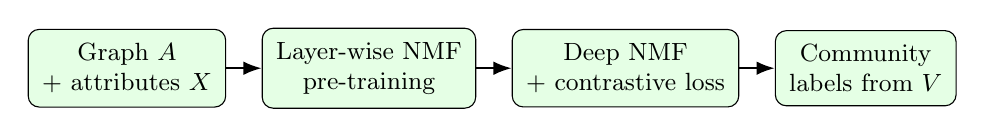
\begin{tikzpicture}[
  box/.style={draw, rounded corners, align=center, font=\small, inner sep=5pt, fill=green!10},
  arr/.style={-{Latex}, thick}
]
\node[box] (data) {Graph $A$\\+ attributes $X$};
\node[box, right=0.45cm of data] (pre) {Layer-wise NMF\\pre-training};
\node[box, right=0.45cm of pre] (cd) {Deep NMF\\+ contrastive loss};
\node[box, right=0.45cm of cd] (out) {Community\\labels from $V$};
\draw[arr] (data) -- (pre);
\draw[arr] (pre) -- (cd);
\draw[arr] (cd) -- (out);
\end{tikzpicture}

\vspace{8pt}
\begin{columns}[T]
\column{0.52\textwidth}
\textbf{Datasets}
\begin{itemize}
    \item \textbf{Cora}: 2708 nodes, 7 classes
    \item \textbf{Citeseer}: 3312 nodes, 6 classes
    \item \textbf{PubMed}: 19717 nodes, 3 classes
\end{itemize}

\column{0.48\textwidth}
\textbf{Loss terms}
\begin{itemize}
    \item Reconstruct $A$ and $X$
    \item Contrastive (two views)
    \item Laplacian regularizer
    \item Non-negativity penalty
\end{itemize}
\end{columns}

\vspace{5pt}
\small
Paper settings kept: Cora 550 ep, Citeseer 1000 ep, PubMed 600 ep; $\tau$ and loss weights from the official config.
\end{frame}

% ----------------------------------------
% SLIDE 3: REPRODUCTION
% ----------------------------------------
\begin{frame}{\textbf{Reproduction / Implementation}}

\textbf{Setup}
\begin{itemize}
    \item Google Colab, Tesla T4, PyTorch
    \item Three notebooks: Cora, Citeseer, PubMed
    \item Metrics: \textbf{ACC} and \textbf{NMI} (paper Table 1)
\end{itemize}

\vspace{3pt}
\textbf{Unchanged from the paper}
\begin{itemize}
    \item Layer shapes, learning rate, $\tau$, contrastive / reconstruction weights
    \item NMF pre-training, then contrastive fine-tuning
\end{itemize}

\vspace{3pt}
\textbf{Changes we made}
\begin{itemize}
    \item Citeseer / PubMed ship without \texttt{walks.txt} $\rightarrow$ walks optional
    \item PubMed OOM: $N{=}19717$ contrastive matrices were ${\sim}1.45$\,GiB each
    \item Fix: chunked similarity; no extra dense $N\times N$ tensors
    \item PubMed: \textbf{1 run} (20-run mean did not finish on T4)
\end{itemize}
\end{frame}

% ----------------------------------------
% SLIDE 4: RESULTS TABLE
% ----------------------------------------
\begin{frame}{\textbf{Results \& Comparison}}

\begin{table}
\centering
\scriptsize
\begin{tabular}{lccccc}
\toprule
\textbf{Dataset} & \textbf{Paper ACC} & \textbf{Ours ACC} & \textbf{Paper NMI} & \textbf{Ours NMI} & \textbf{Runs} \\
\midrule
Cora     & 0.6081 & $0.6006 \pm 0.016$ & 0.4006 & $0.3942 \pm 0.026$ & 20 \\
Citeseer & 0.4756 & $0.4700 \pm 0.025$ & 0.2559 & $0.2500 \pm 0.021$ & 20 \\
PubMed   & 0.6653 & 0.6600            & 0.2330 & 0.2232            & 1 \\
\bottomrule
\end{tabular}
\end{table}

\vspace{8pt}
\begin{itemize}
    \item Cora and Citeseer sit within ${\sim}1$ ACC point of Table 1 (20-run mean).
    \item PubMed 0.660 vs 0.665 on one 600-epoch run.
    \item Pretrain-only ACC was much lower --- fine-tuning is the real gain.
\end{itemize}
\end{frame}

% ----------------------------------------
% TRAINING CURVES FROM THE THREE NOTEBOOKS
% ----------------------------------------
\begin{frame}{\textbf{Training Curves --- Cora}}
\centering
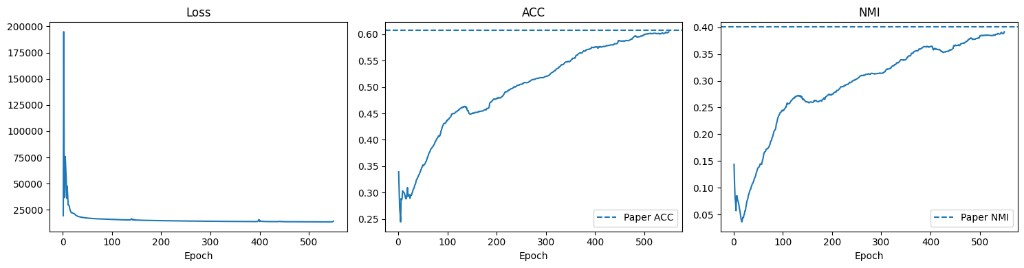
\includegraphics[width=0.98\textwidth]{cora_curves.png}\\[2pt]
{\scriptsize Directly from \texttt{Lab1CDNMF\_Colab\_1} (550 epochs). Dashed line = paper Cora ACC 0.6081, NMI 0.4006.}
\end{frame}

\begin{frame}{\textbf{Training Curves --- Citeseer}}
\centering
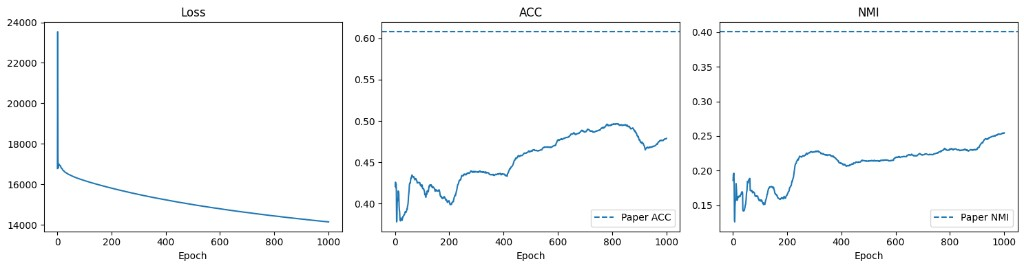
\includegraphics[width=0.98\textwidth]{citeseer_curves.png}\\[2pt]
{\scriptsize Directly from \texttt{Lab1CDNMF\_Colab\_2} (1000 epochs). Table 1 Citeseer: ACC 0.4756, NMI 0.2559.}
\end{frame}

\begin{frame}{\textbf{Training Curves --- PubMed}}
\centering
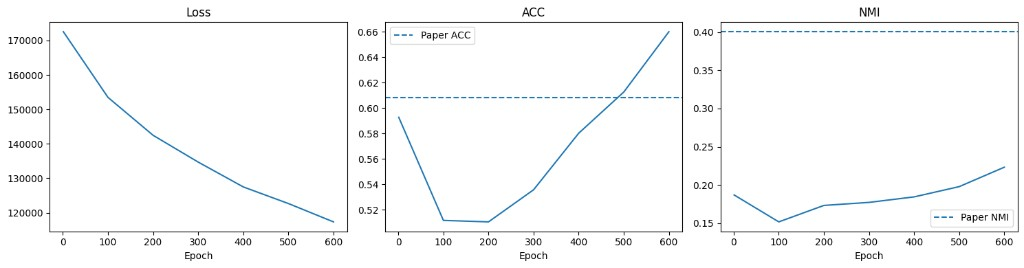
\includegraphics[width=0.98\textwidth]{pubmed_curves.png}\\[2pt]
{\scriptsize Directly from \texttt{Lab1CDNMF\_Colab\_3} (600 epochs). Table 1 PubMed: ACC 0.6653, NMI 0.2330.}
\end{frame}

% ----------------------------------------
% SLIDE 5: CONCLUSION
% ----------------------------------------
\begin{frame}{\textbf{Conclusion \& Learning}}

\begin{itemize}
    \item CDNMF was reproduced on Cora, Citeseer, and PubMed.
    \item ACC/NMI land in the paper's band; curves show loss falling and ACC/NMI rising toward Table 1.
    \item Remaining gap is small (${\sim}0.005$--$0.01$); PubMed used 1 run, not 20.
    \item Hard parts: missing \texttt{walks.txt}, PubMed CUDA OOM, 20-run time on T4.
    \item Next: full 20-run PubMed on a larger GPU; sparse adjacency on device.
    \item Takeaway: paper hyperparameters + pre-training + contrastive fine-tuning are all required.
\end{itemize}
\end{frame}

% ----------------------------------------
% THANK YOU
% ----------------------------------------
\begin{frame}
\centering
\Huge \textbf{Thank You!}
\end{frame}

\end{document}
